\documentclass{article}

\usepackage{graphicx}
\usepackage{url}
 
\begin{document}

\title{AI Coffe Club (11/12/2019)\\ Normalization}
\date{}

\maketitle

\begin{center}
Last modification: \today\\
\end{center}

\section{Why is Normalization Important?}

Consider a simple scenario in which the neural network takes two inputs (let's say $x_0$ and $x_1$) and such variables have significantly different ranges $x_0 = [0, 1]$ and $x_1 = [0, 10]$. The goal of the network is to learn a set of weights to combine such inputs throuh linear combinations and non-linear activations. This implies that the weights associated to each input will belong to different ranges.

Such phenomena has a direct impact in the topology of the loss function as shown below:

\begin{figure}[!htb]
  \centering
  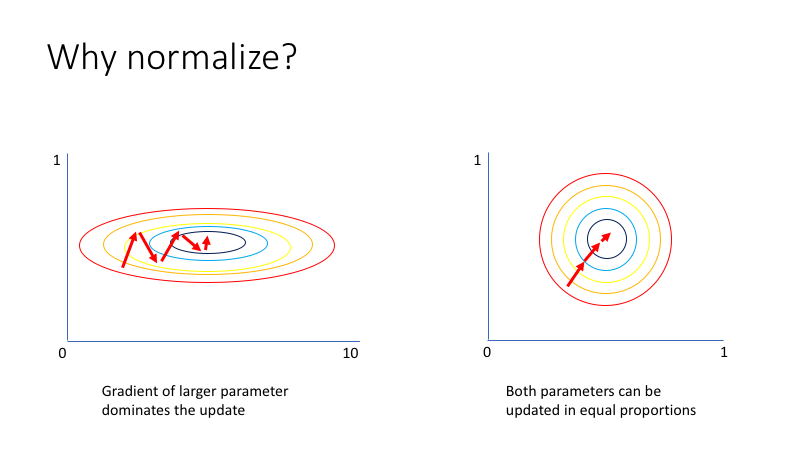
\includegraphics[clip, trim=0 100 0 0, width=\linewidth]{normalization.png}
\end{figure}

This will indirectly lead to the network placing more emphasis on specific parameter gradients just because they produce larger activations. This fact makes training harder and hurts convergence which in turn leads to needing more iterations to train a network properly.

\section{How to Normalize the Input}

An easy way to avoid this problem is to normalize the input to have zero mean and unit variance using the standardization approach (putting the data in the range $[-1, 1]$).

In some cases, standardization can hurt performance depending on the activation layers. For instance, ReLU activations tend to show better performance if the data is just scaled to the $[0, 1]$ range instead of standardized to $[-1, 1]$.

\section{How to Normalize between Layers}

The aforementioned approach solves the problem of normalizing the input but that only affects significantly the first layers of the network. Unfortunately, the distribution of each layer's input changes during training since the weights from the previous layers change as we iterate through the training set.

This leads to slower training (requiring lower learning rates to reach convergence), requires careful initialization, and makes it really hard to train certain models with saturating non-linearities. This problem is named internal covariance shift.

However, knowing that input normalization helps, this intuition can be extended to the whole network to help it learn more effectively by making normalization a part of the architecture.

We would like to normalize the activations of a given layer so that we improve the learning of the weights that connect to the next layer. This technique is known as batch normalization \footnote{\url{https://arxiv.org/pdf/1502.03167.pdf}}.

There is a debate whether to normalize the input sum $z$ or the activations $a$, but in practice most people normalize the input sum.

Considering $z^l_i$ (the input sum from a layer $l$ for each observation of the batch $i$, we compute the batch mean $\mu^l_{\mathcal{B}}$ and variance ${\sigma^2}^l_{\mathcal{B}}$:

\begin{equation}
\mu^l_{\mathcal{B}} = \frac{1}{m}\sum^m_{i=0}z^l_i
\end{equation}

\begin{equation}
{\sigma^2}^l_{\mathcal{B}} = \frac{1}{m}\sum^m_{i=0}(z^l_i - \mu^l_{\mathcal{B}})^2
\end{equation}

Using those values, we can normalize the input sums to have zero mean and unit variance as follows:

\begin{equation}
{z^l_i}_{norm} = \frac{z^l_i - \mu^l_\mathcal{B}}{\sqrt{{\sigma^2}^l_{\mathcal{B}}+ \epsilon}}
\end{equation}

(Note that a small $\epsilon$ is added for numerical reasons to avoid a possible division by zero).

Nevertheless, in some cases we don't want to explicitly normalize to zero mean and unit variance (this is actually bad for some activation functions such as sigmoid) but rather we allow the network to learn the optimal distribution by scaling the normalized values by $\gamma$ and shifting by $\beta$:

\begin{equation}
\hat{z}^l_i = \gamma {z^l_i}_{norm} + \beta
\end{equation}

(Note: $\gamma$ and $\beta$ are learned parameters which are used across all batches).

\end{document}